\documentclass{beamer}
\usetheme{Warsaw}

\usepackage[utf8]{inputenc}
\usepackage{fancybox}
\usepackage{multimedia} 
\usepackage{subfig}
\usepackage{amsmath}
\usepackage{hyperref}
\usepackage[all]{xy}
\begin{document}


\title[Stochastik] % (optional, only for long titles)
{Stochastik für Informatiker
\\
\includegraphics[scale=0.5]{img/craps}
}
\subtitle{}
\author[Dr. Johannes Riesterer] % (optional, for multiple authors)
{Dr.  rer. nat. Johannes Riesterer}

\date[KPT 2004] % (optional)
{}

\subject{Stochastik}


\frame{\titlepage}






\begin{frame}
    \frametitle{Statistik - Parameterschätzung}
\framesubtitle{}

\begin{block}{Erraten des Bereichs von Zufallsvariablen}
Angenommen man findet einen Apparat (Fluxkompensator?), der zufällig Zahlen in einem Intervall $[0, \rho]$ ausgibt. Anhand von Beobachtungen der Zahlen möchte man $\rho$ schätzen.
\end{block}

\begin{figure}[htp]
      \centering
    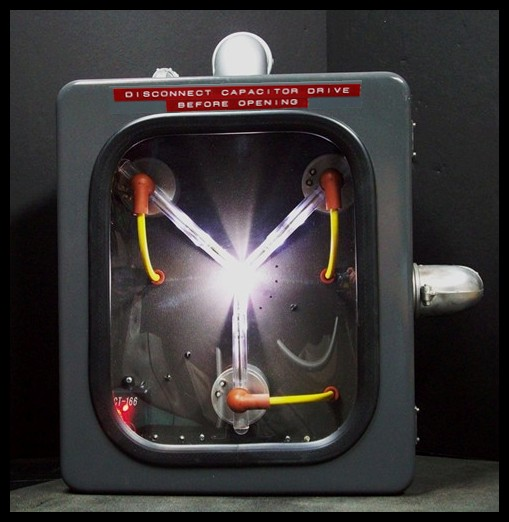
\includegraphics[width=0.35\textwidth]{img/flux}
      \caption{Quelle: forevergeek}
\end{figure}
 \end{frame}


\begin{frame}
    \frametitle{Statistik - Parameterschätzung}
\framesubtitle{}

\begin{block}{Erraten des Bereichs von Zufallsvariablen - Modell}
 Wir machen die Annahme, dass alle Zahlen in dem Intervall gleich wahrscheinlich auftreten und  nehmen $n$ Stichproben $X_1, \cdots, X_n$.
Einen Schätzer für $\rho$ bezeichnen wir mit $T_n$.
\end{block}

\begin{block}{Erraten des Bereichs von Zufallsvariablen - Schätzer 1}
Eine einfache und einleuchtende Idee ist es, $\rho$ durch die größte beobachtete Zahl zu schätzen, also
$T_n^{max} := \max(X_1, \cdots, X_n)$.
 \end{block}

\begin{block}{Erraten des Bereichs von Zufallsvariablen - Schätzer 2}
Da das Auftreten der Zahlen gleich wahrscheinlich ist, ist der Erwartungswert des Zufallsexperiments $\rho /2$. Unter Berufung auf das  schwache Gesetz der Großen Zahlen erscheint der Schätzer
$T_n^{E} :=  2 \cdot \biggl( \frac{1}{n} \sum_{i=1}^n X_i \biggr)$ sehr plausibel.
 \end{block}

 \end{frame}




\begin{frame}
    \frametitle{Statistik - Parameterschätzung}
\framesubtitle{}

\begin{block}{Erraten des Bereichs von Zufallsvariablen - Vergleich}
Welcher Schätzer ist besser und in welchem Sinn?
\end{block}

\begin{block}{Erraten des Bereichs von Zufallsvariablen - Vergleich Konvergenz $T_n^{max}$}
\begin{align*}
& P(| T_n^{max} - \rho | \geq \epsilon)   \\
& = P(T_n^{max} \leq \rho - \epsilon \text{ oder } T_n^{max} \geq \rho + \epsilon)   \\
& = P(T_n^{max} \leq \rho - \epsilon) + \underbrace{P(T_n^{max} \geq \rho + \epsilon)}_{= \, 0, \text{ da } T_n^{max} \leq \rho}   
\end{align*}
\end{block}

 \end{frame}


\begin{frame}
    \frametitle{Statistik - Parameterschätzung}
\framesubtitle{}

\begin{block}{Erraten des Bereichs von Zufallsvariablen - Vergleich Konvergenz $T_n^{max}$ (Forts.)}
\begin{align*}
& = P(T_n^{max} \leq \rho - \epsilon)   \\
& = P(X_1  \leq \rho - \epsilon, \cdots,  X_n \leq \rho - \epsilon )  = \left(\frac{\rho - \epsilon}{\rho}\right)^n \underset{n \to \infty}{\longrightarrow} 0
\end{align*}
\end{block}


\begin{block}{Erraten des Bereichs von Zufallsvariablen - Vergleich Konvergenz $T_n^{E}$}
\begin{align*}
& P(| T_n^{E} - \rho | \geq \epsilon)   = P(| \frac{1}{n} \sum X_i  - \frac{\rho}{2} | \geq \frac{\epsilon}{2})  \underset{n \to \infty}{\longrightarrow} 0 \\
 & \text{(Gesetz der Großen Zahlen)}
\end{align*}
\end{block}

 \end{frame}


\begin{frame}
    \frametitle{Statistik - Parameterschätzung}
\framesubtitle{}


\begin{block}{Verteilungsfunktion von $T_n^{max}$}
Da die $X_i$ u.i.v. und gleichverteilt auf $[0, \rho]$ sind, gilt für $0 \leq c \leq \rho$:
\begin{align*}
P( T_n^{max}  \leq c) & = P(\max(X_1, \cdots, X_n) \leq c) \\
& = P(X_1 \leq c, \cdots, X_n \leq c) \\
& \overset{\text{u.i.v.}}{=} \prod_{i=1}^n P(X_i \leq c) = \left(\frac{c}{\rho}\right)^n
\end{align*}
\end{block}

 \end{frame}


\begin{frame}
    \frametitle{Statistik - Parameterschätzung}
\framesubtitle{}

\begin{block}{Dichte und Erwartungswert von $T_n^{max}$}
Die Dichte ergibt sich als Ableitung der Verteilungsfunktion:
$f_{T_n^{max}}(x) = \frac{d}{dx} \left(\frac{x}{\rho}\right)^n = \frac{n}{\rho^n} x^{n-1}$. Damit:
\begin{align*}
\mathbb{E}(T_n^{max} ) & = \int_{0}^{\rho} x \cdot \frac{n}{\rho^n} x^{n- 1} \; dx  = \frac{n}{\rho^n} \int_{0}^{\rho} x^n \; dx = \frac{n}{n+1} \rho    \underset{n \to \infty}{\longrightarrow} \rho
\end{align*}
\end{block}

\begin{block}{Erwartungswert von $T_n^{E}$}
\begin{align*}
& \mathbb{E}(T_n^{E} ) = \frac{2}{n} \sum \mathbb{E}(X_i)   = \rho
\end{align*}
\end{block}
 \end{frame}




\begin{frame}
    \frametitle{Statistik - Parameterschätzung}
\framesubtitle{}

\begin{block}{Erraten des Bereichs von Zufallsvariablen - Vergleich Varianz}
\begin{align*}
& \mathbb{V}(T_n^{E} ) = \frac{4}{n} \mathbb{V}(X_1)   =  \frac{4}{n \rho}   \int_{0}^{\rho } (x - \frac{\rho}{2})^2 \; dx = \frac{\rho^2}{3n}
\end{align*}
\end{block}
\begin{block}{Erraten des Bereichs von Zufallsvariablen - Vergleich Varianz}
\begin{align*}
& \mathbb{V}(T_n^{max} ) = \mathbb{E}((T_n^{max})^2 ) - (\mathbb{E}(T_n^{max} ))^2   \\
& = \int_{0}^{\rho} x^2 \frac{n}{\rho^n} x^{n- 1} \; dx - (\frac{n \rho}{n+1})^2 = \frac{n \rho^2}{(n+1)^2 (n+2)} 
\end{align*}
\end{block}
 \end{frame}




% \begin{frame}
  %  \frametitle{Statistik - Parameterschätzung}
%\framesubtitle{}
%\includegraphics[scale=0.08]{img/schätzer.png}
 %\end{frame}




\begin{frame}
    \frametitle{Statistik - Parameterschätzung}
\framesubtitle{}

\begin{block}{Statistisches Modell}
Ein statistisches Modell ist ein Tripel $(\mathcal{X}, \mathcal{F}, P_\rho :  \rho \in \Theta)$ bestehend aus einer $\sigma$-Algebra $\mathcal{F}$ über dem Grundraum $\mathcal{X}$ und einer indizierten Menge (mit mindestens zwei Elementen) von Maßen $\{ P_\rho\}_{\rho \in \Theta}$. Für $\Theta \subset \mathbb{R}^n$ bezeichnet man es auch als parametrisiertes statistisches Modell. 
\end{block}

\begin{block}{Beispiel: Fluxkompensator}
\begin{itemize}
\item $\mathcal{X} = [0, \rho]^n$ (Raum aller möglichen $n$-Stichproben)
\item $\mathcal{F} = \mathcal{B}([0,\rho]^n)$ (Borel-$\sigma$-Algebra)
\item $P_\rho = \mathcal{U}([0,\rho])^{\otimes n}$ ($n$-faches Produkt der Gleichverteilung)
\item $\Theta = (0, \infty)$ (der unbekannte Parameter $\rho$)
\end{itemize}
\end{block}
 \end{frame}


\begin{frame}
    \frametitle{Statistik - Parameterschätzung}
\framesubtitle{}

\begin{block}{Statistik}
Sei   $(\mathcal{X}, \mathcal{F}, P_\rho :  \rho \in\Theta)$ ein statistisches Modell und $(\Sigma, \mathcal{G})$ eine $\sigma$-Algebra über $\Sigma$. Eine Zufallsvariable 
\begin{align*}
X : \mathcal{X} \to \Sigma
\end{align*}
wird Statistik für  $(\mathcal{X}, \mathcal{F}, P_\rho :  \rho \in \Theta)$  genannt.
\end{block}
 \end{frame}



\begin{frame}
    \frametitle{Statistik - Parameterschätzung}
\framesubtitle{}

\begin{block}{Schätzer}
Sei   $(\mathcal{X}, \mathcal{F}, P_\rho :  \rho \in \Theta)$ ein statistisches Modell, $(\Sigma, \mathcal{G})$ eine $\sigma$-Algebra über $\Sigma$ und  
\begin{align*}
& \tau : \Theta \to \Sigma \\
 & \rho \mapsto \tau(\rho) 
\end{align*}
eine Abbildung. Eine Statistik   $T: \mathcal{X} \to \Sigma$  wird Schätzer für $\tau$ genannt.
\end{block}

\begin{block}{Beispiel: Fluxkompensator}
\begin{itemize}
\item Zielraum: $\Sigma = (0, \infty)$, zu schätzende Abbildung: $\tau(\rho) = \rho$ (Identität)
\item $T_n^{max}(x_1, \cdots, x_n) = \max(x_1, \cdots, x_n)$ ist ein Schätzer für $\tau$
\item $T_n^{E}(x_1, \cdots, x_n) = \frac{2}{n} \sum_{i=1}^n x_i$ ist ein Schätzer für $\tau$
\end{itemize}
\end{block}
 \end{frame}


\begin{frame}
    \frametitle{Statistik - Parameterschätzung}
\framesubtitle{}

\begin{block}{Konsistenz}
Eine Schätzfolge $T_n: \mathcal{X} \to \Sigma$  heißt konsistent, falls
\begin{align*}
P( |T_n - \tau(\rho)  |  \geq \epsilon)  \underset {n \to \infty}{\longrightarrow} 0 \text{ für alle } \epsilon > 0 \text { und alle } \rho \in \Theta  
\end{align*}
also $T_n \to \tau(\rho)$ für $n \to \infty$  (stochastisch).
\end{block}
\begin{block}{Erwartungstreue}
Ein Schätzer $T: \mathcal{X} \to \Sigma$  heißt Erwartungstreu (unbiased), falls
\begin{align*}
\mathbb{E}(T) = \tau(\rho) \text{ für alle } \rho \in \Theta.
\end{align*}
Andernfalls heißt $\mathbb{E}(T) - \tau(\rho) $ der Bias oder der systematische Fehler.
\end{block}
 \end{frame}


\begin{frame}
    \frametitle{Statistik - Parameterschätzung}
\framesubtitle{}

\begin{block}{Beispiel: Fluxkompensator -- Konsistenz und Erwartungstreue}
\begin{itemize}
\item $T_n^{max}$ ist konsistent: $P(|T_n^{max} - \rho| \geq \epsilon) = \left(\frac{\rho - \epsilon}{\rho}\right)^n \to 0$
\item $T_n^{max}$ ist \textbf{nicht} erwartungstreu: $\mathbb{E}(T_n^{max}) = \frac{n}{n+1}\rho \neq \rho$
\item $T_n^{max}$ ist jedoch \textbf{asymptotisch erwartungstreu}: $\mathbb{E}(T_n^{max}) = \frac{n}{n+1}\rho \underset{n \to \infty}{\longrightarrow} \rho$
\item $T_n^{E}$ ist konsistent (nach GGZ)
\item $T_n^{E}$ ist erwartungstreu: $\mathbb{E}(T_n^{E}) = \rho$
\end{itemize}
\end{block}
 \end{frame}

\begin{frame}
    \frametitle{Statistik - Parameterschätzung}
\framesubtitle{}
\begin{block}{Stichprobenmittel und  Stichprobenvarianz}
\begin{itemize}
\item Für $n \geq 2$ sei  $\biggl ( \mathbb{R}^n, \mathcal{B}(\mathbb{R}^n ), P^n_\rho :=  \prod (P_\rho)_i \biggr)$ das Produktmodell
\item $X_i(x_1, \cdots , x_n) = x_i$ die Projektion auf die $i$-te Koordinate  
\item $m(\rho) =  \mathbb{E}(X_i) $ so wie $v(\rho) =\mathbb{V}(X_i)$. 
\item  $M= \frac{1}{n} \sum_{i=1}^n X_i$ Stichprobenmittel  und $V= \frac{1}{n-1} \sum_{i=1}^n (X_i - M)^2$ Stichprobenvarianz.
\end{itemize}

 Dann sind $M$  und $V$ erwartungstreue Schätzer für $m:=$ bzw. $v$.

\end{block}

\begin{block}{Beweis}
Sei $\rho \in \Theta$ fest. Wegen linearität des EW und u.i.v. ist $\mathbb{E}(M) =\frac{1}{n} \sum_{i=1}^n \mathbb{E}(X_i) = m(\rho) $.
\end{block}


 \end{frame}


\begin{frame}
    \frametitle{Statistik - Parameterschätzung}
\framesubtitle{}

\begin{block}{Beweis}
Aus Linearität des EW und $\mathbb{E}(X_i - M) = 0$, u.i.v, stochastische Unabhängigkeit folgt
\begin{align*}
&(n-1) \mathbb{E}(V)  = \sum_{i=1}^n  \mathbb{V}(X_i - M) \\
& = n   \mathbb{V} (\frac{n-1}{n} X_1  - \frac{1}{n} \sum_{j=2}^n X_j) \\
& = n((\frac{n-1}{n})^2 + (n-1) \frac{1}{n^2}  ) v(\rho) = (n-1) v(\rho)
\end{align*}
Durch Teilen beider Seiten durch $n-1$ folgt die Behauptung. 
\end{block}


 \end{frame}




\begin{frame}
    \frametitle{Statistik - Parameterschätzung}
\framesubtitle{}

\begin{block}{Likelyhood Funktion}
Für eine parametrisierte Dichte $p_\rho : \mathcal{X}   \to  [0,1]$ heißt 
\begin{align*}
& p_x  : \Theta   \to  [0,1] \\
& p_x(\rho):=  p(x, \rho) 
\end{align*}
die Likelihood Funktion zum Beobachtungswert $x \in \mathcal{X}$.

\end{block}
 \end{frame}



\begin{frame}
    \frametitle{Statistik - Parameterschätzung}
\framesubtitle{}
\begin{block}{Maximum Likelihood Schätzer}
Ein Schätzer $T: \mathcal{X} \to \Sigma$ heißt Maximum-Likelihood-Schätzer
 bezüglich des Beobachtungswerte $x \in \mathcal{X}$, falls
\begin{align*}
p_x(T(x)) = \max_{\rho \in \Theta} p_x (\rho) 
\end{align*}
also der Schätzwert $T(x)$ eine Maximalstelle der Funktion  $p_x$ auf $\Theta$ ist.
\end{block}
\begin{center}
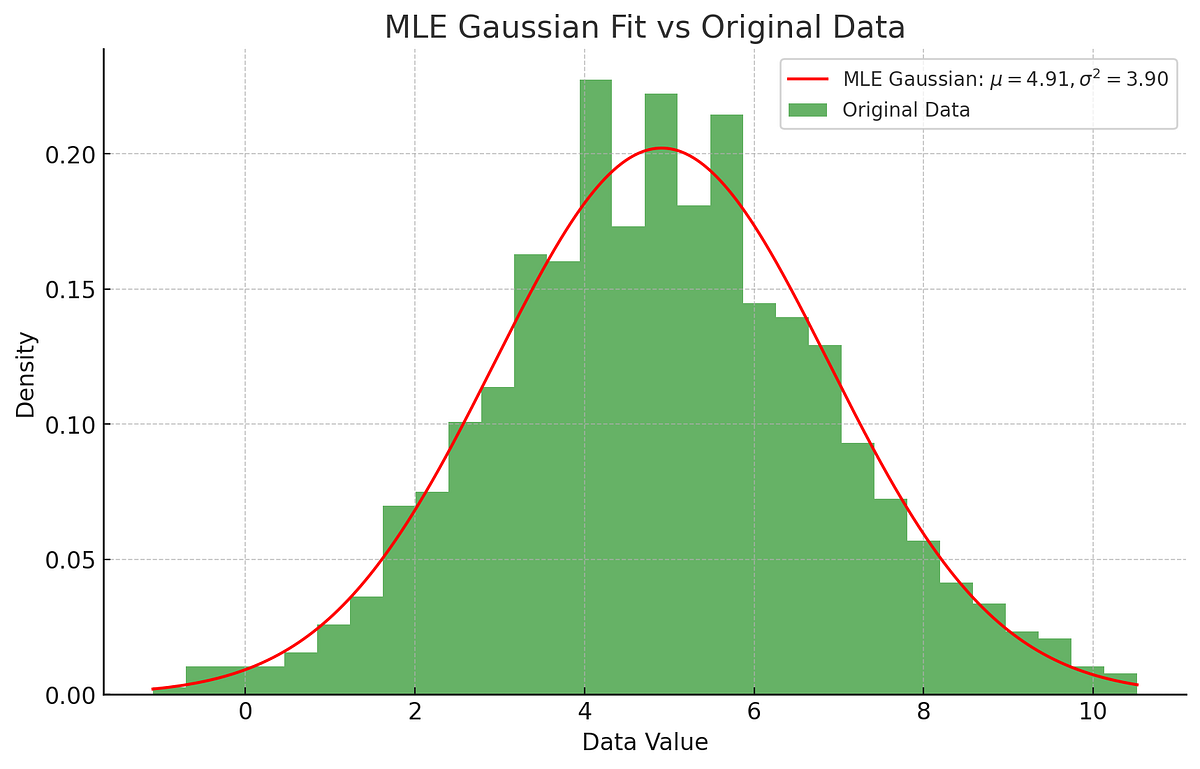
\includegraphics[scale=0.15]{img/maximumlikelyhood.png}    
\end{center}
 \end{frame}


 
\begin{frame}
    \frametitle{Statistik - Parameterschätzung}
\framesubtitle{}
\begin{block}{Intuition: Maximum Likelihood}
\textbf{Idee:} Wähle den Parameter $\rho$, unter dem die beobachteten Daten $x$ am \textbf{wahrscheinlichsten} sind.
\begin{itemize}
\item $x = (x_1, \ldots, x_n) \in \mathcal{X}$ ist die \textbf{konkrete Stichprobe} (beobachtete Daten, fest)
\item Die Dichte $p_\rho(x)$ gibt an, wie ``plausibel'' die Beobachtung $x$ unter dem Parameter $\rho$ ist
\item Beim ML-Schätzer vertauschen wir die Perspektive: Wir fixieren $x$ und variieren $\rho$
\item Gesucht ist das $\rho$, das $p_x(\rho) = p(x, \rho)$ maximiert
\end{itemize}
\end{block}

 \end{frame}


\begin{frame}
    \frametitle{Statistik - Parameterschätzung}
\framesubtitle{}
\begin{block}{Stichproben in der formalen Sprache}
\begin{itemize}
\item $\mathcal{X} = \mathbb{R}^n$: Stichprobenraum (alle möglichen Beobachtungen)
\item $X_i : \mathcal{X} \to \mathbb{R}$: Zufallsvariable (Projektion auf $i$-te Koordinate)
\item $x = (x_1, \ldots, x_n) \in \mathcal{X}$: konkrete \textbf{Realisierung} = Stichprobe
\end{itemize}
\textbf{Wichtig:} In $p_x(\rho)$ ist $x$ \textbf{fest} (schon beobachtet). Nur $\rho$ wird variiert -- deshalb ist $p_x$ eine Funktion von $\rho$ allein.
\end{block}

 \end{frame}


\begin{frame}
    \frametitle{Statistik - Parameterschätzung}
\framesubtitle{}
\begin{block}{Maximum Likelihood -- Erklärung}
Äquivalente Schreibweise: $T(x) \in \arg\max_{\rho \in \Theta} \, p_x(\rho)$

$\arg\max$ einer Funktion $f: A \to \mathbb{R}$ ist der \textbf{Eingabewert}, bei dem $f$ ihr Maximum annimmt:
$\arg\max_{a \in A} f(a) = \{ a \in A : f(a) \geq f(a') \text{ für alle } a' \in A \}$
\end{block}

\begin{block}{Maximum Likelihood -- Produkt, nicht Summe}
Für u.i.v. Stichproben $x = (x_1, \cdots, x_n)$ ist die Likelihood das \textbf{Produkt} der Einzeldichten (wegen Unabhängigkeit):
\begin{align*}
p_x(\rho) = \prod_{i=1}^n p_\rho(x_i)
\end{align*}
Man sucht das $\rho$, das dieses Produkt maximiert.
\end{block}

 \end{frame}


\begin{frame}
    \frametitle{Statistik - Parameterschätzung}
\framesubtitle{}
\begin{block}{ML-Schätzer: Kompromiss über alle Datenpunkte}
\textbf{Beispiel:} $X_1, X_2 \sim N(m, 1)$, beobachtet: $x_1 = 2,\; x_2 = 8$.
\begin{itemize}
\item $m = 2$: $p_m(x_1)$ groß, $p_m(x_2)$ winzig $\Rightarrow$ Produkt klein
\item $m = 8$: $p_m(x_2)$ groß, $p_m(x_1)$ winzig $\Rightarrow$ Produkt klein
\item $m = 5$: beide moderat $\Rightarrow$ \textbf{Produkt maximal}
\end{itemize}
Der ML-Schätzer findet den \textbf{besten Kompromiss} über alle Datenpunkte -- nicht den besten Parameter für einen einzelnen Wert.
\end{block}

 \end{frame}


\begin{frame}
    \frametitle{Statistik - Parameterschätzung}
\framesubtitle{}
\begin{block}{ML bei abhängigen Daten}
Im allgemeinen Fall (ohne Unabhängigkeit) gilt die Kettenregel:
\begin{align*}
p_\rho(x_1, \ldots, x_n) = p_\rho(x_1) \cdot p_\rho(x_2 \mid x_1) \cdot p_\rho(x_3 \mid x_1, x_2) \cdots
\end{align*}
Bei Unabhängigkeit vereinfacht sich $p_\rho(x_i \mid x_1, \ldots, x_{i-1}) = p_\rho(x_i)$ und man erhält das Produkt.
\end{block}

\begin{block}{Interpretation}
\begin{itemize}
\item Unabhängig: ``Wie wahrscheinlich ist jeder Wert einzeln?''
\item Abhängig: ``Wie wahrscheinlich ist dieser Wert, \textbf{gegeben} die vorherigen?''
\end{itemize}
In dieser Vorlesung arbeiten wir stets mit u.i.v., also reicht das Produkt.
\end{block}

 \end{frame}



\begin{frame}
    \frametitle{Statistik - Parameterschätzung}
\framesubtitle{}
\begin{block}{Erraten des Bereichs -- Likelihood-Funktion}
Die $X_i$ sind u.i.v. gleichverteilt auf $[0, \rho]$ mit Dichte $\frac{1}{\rho}$. Für eine Stichprobe $x = (x_1, \cdots, x_n)$:
\begin{align*}
p_x (\rho) = \prod_{i=1}^n \frac{1}{\rho} \cdot \mathbf{1}_{[0,\rho]}(x_i) =  \begin{cases}  \frac{1}{\rho^n}  & \text{falls }  x_1, \cdots , x_n \leq \rho  \\  0  & \text{sonst}\end {cases}
\end{align*}
\end{block}

\begin{block}{Erraten des Bereichs -- Maximierung}
\begin{itemize}
\item $p_x(\rho) = 0$ für $\rho < \max(x_1, \cdots, x_n)$ (Daten wären unmöglich)
\item $p_x(\rho) = \frac{1}{\rho^n}$ für $\rho \geq \max(x_1, \cdots, x_n)$ (fällt monoton in $\rho$)
\item Maximum bei kleinstem zulässigem $\rho$: $T_n^{max}(x) = \max(x_1, \cdots, x_n)$
\end{itemize}
\end{block}

 \end{frame}




\begin{frame}
    \frametitle{Statistik - Parameterschätzung}
\framesubtitle{}
\begin{block}{Physikalische Messung - Maximum Likelyhood-Schätzer}
Gegeben ist ein Sensor mit einer unbekannten Messgenauigkeit. Wir nehmen deshalb an, dass die Messung des Sensors einer Normalverteilung folgt, 
wobei der Erwartungswert (Messwert) und die Varianz (Streuung um Messwert) unbekannt sind. Wir machen $n$ unabhängige Messungen und erhalten damit das Normalverteilte Produktmodell $\bigl(\mathbb{R}^n, \mathcal{B}(\mathbb{R}^n), \prod_{i=1}^n N(m,v): m \in \mathbb{R}, v  >0 \bigr)$. 

\end{block}

 \end{frame}



\begin{frame}
    \frametitle{Statistik - Parameterschätzung}
\framesubtitle{}
\begin{block}{Physikalische Messung - Maximum Likelyhood-Schätzer}
Die Likelihood-Funktion ist gegeben durch
\begin{align*}
p_x(\rho) =  \prod_{i=1}^n \frac {1}{ \sqrt{2 \pi v }} e^{- \frac{(x_i- m)^2}{ 2v}} =  \frac {1}{ \sqrt{2 \pi v }} e^{- \sum_{i=1}^n \bigl( \frac{(x_i- m)^2}{ 2v} \bigr)} 
\end{align*} 
mit $x = (x_1, \cdots, x_n)$ und $\rho=(m,v)$.
\end{block}

\begin{block}{Physikalische Messung - Maximum Likelyhood-Schätzer}
Um diesen Ausdruck zu maximieren, muss $m$ so gewählt werden, dass die quadratische Fehlersumme $ \sum_{i=1}^n (x_i- m)^2$ minimal wird.  Das ist der Fall für $m= M(x)= \frac{1}{n} \sum_{i=1}^n x_i$.
\end{block}

 \end{frame}

\begin{frame}
    \frametitle{Statistik - Parameterschätzung}
\framesubtitle{}
\begin{block}{Physikalische Messung - Maximum Likelyhood-Schätzer}
Des weiteren muss $v$ so gewählt werden, dass $ \frac {1}{ \sqrt{2 \pi v }} e^{- \sum_{i=1}^n \bigl( \frac{(x_i- M(x))^2}{ 2v} \bigr)}$ maximal wird. Differenziert man den Logarithmus dieses Ausdrucks nach $v$, erhalten wir
\begin{align*}
& -\frac{d}{dv} (\frac{n}{2} \log(v) + \frac{1}{2v} \sum_{i=1}^n (x_i - M(x))^2 ) \\
& = -\frac{n}{2v} + \frac{1}{2v^2}\sum_{i=1}^n (x_i - M(x))^2 
\end{align*}
Dieser Term ist maximal, falls der letzte Term verschwindet. Dies ist er Fall für
$v = V(x) =\frac{1}{n}\sum_{i=1}^n (x_i - M(x))^2$
\end{block}

 \end{frame}















\end{document}
